% Flowchart / architecture diagram template
% Compile with: pdflatex flowchart-template.tex
\documentclass[border=10pt]{standalone}
\usepackage[T1]{fontenc}
\usepackage{tikz}
\usetikzlibrary{positioning, arrows.meta, shapes.geometric, fit, calc, shadows.blur}
\usepackage{xcolor}

\definecolor{accent}{RGB}{60, 120, 200}

\begin{document}
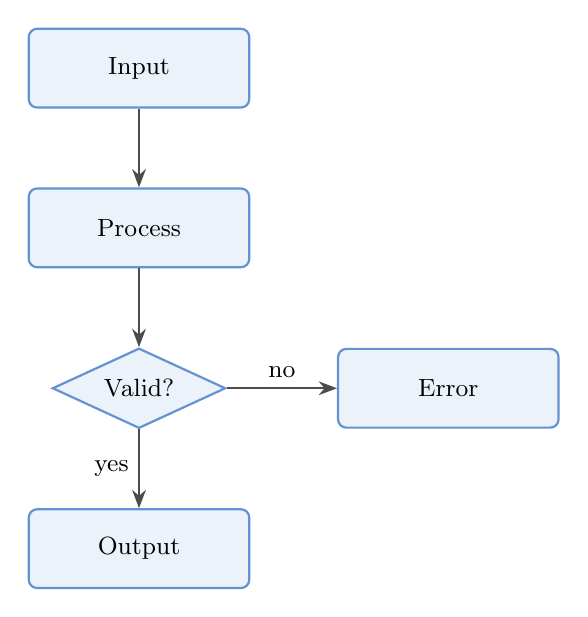
\begin{tikzpicture}[
  node distance=10mm and 14mm,
  every node/.style={font=\small},
  block/.style={
    draw=accent!80, rounded corners=3pt, thick,
    fill=accent!10,
    minimum width=2.8cm, minimum height=1cm,
    align=center,
  },
  decision/.style={
    draw=accent!80, diamond, aspect=2, thick,
    fill=accent!10,
    minimum width=2.2cm, align=center,
  },
  arr/.style={-Stealth, thick, draw=black!70},
]
  \node[block]                       (in)    {Input};
  \node[block, below=of in]          (proc)  {Process};
  \node[decision, below=of proc]     (check) {Valid?};
  \node[block, below=of check]       (out)   {Output};
  \node[block, right=of check]       (err)   {Error};

  \draw[arr] (in)    -- (proc);
  \draw[arr] (proc)  -- (check);
  \draw[arr] (check) -- node[left]  {yes} (out);
  \draw[arr] (check) -- node[above] {no}  (err);
\end{tikzpicture}
\end{document}
